\section{Versuchsaufbau}
\label{sec:Durchführung}

Die Abbildung \ref{abb1} stellt den Versuchsaufbau schematisch dar.
Es handelt sich bei den Halbleiterproben um jene, die nur 
für infrarote Strahlen durchlässig sind, weshalb eine Lichtquelle vorhanden sein 
muss, die entsprechendes Licht erzeugen kann.
Dafür wird eine Halogenlampe verwendet. 
Danach wird das Licht durch Interferenzfilter monochromatisiert und mit Hilfe eines 
Glan-Thompson-Prismas linear polarisiert. Danach wird der Strahl auf die 
Halbleiterprobe gelenkt, welche sich in einem konstanten Magnetfeld im Luftspalt 
eines Elektromagneten befindet. Die Lichtintensität wird schließlich über 
Photowiderstände gemessen. Der Innenwiderstand dieser Elemente ist um mehrere 
Zehnerpotenzen proportional zur Lichtintensität, sodass deutliche 
Rauschspannungen entstehen. Daher wird der Lichtstrahl direkt nach der 
Emittierung durch einen Zerhacker in Einzelpulse geteilt, sodass an den 
Photowiderständen eine Wechselspannung gemessen werden kann. 
Um den Drehwinkel der Polarisationsebene nach dem Durchlauf des Lichtes durch den 
Elektromagneten zu messen, befindet sich hinter ihm ein weiteres Glan-Thompson-Prisma.
Dadurch wird der Strahl geteilt und die Intensität beider Strahlen wird erneut 
über Photowiderstände gemessen und durch einen Differenzverstärker verstärkt,
sodass auf einem danach geschalteten Oszillskop festgestellt werden kann, ob die 
Signalspannungen der Teilstrahlen gleich sind \cite{sample}.

\begin{figure}
    \centering
    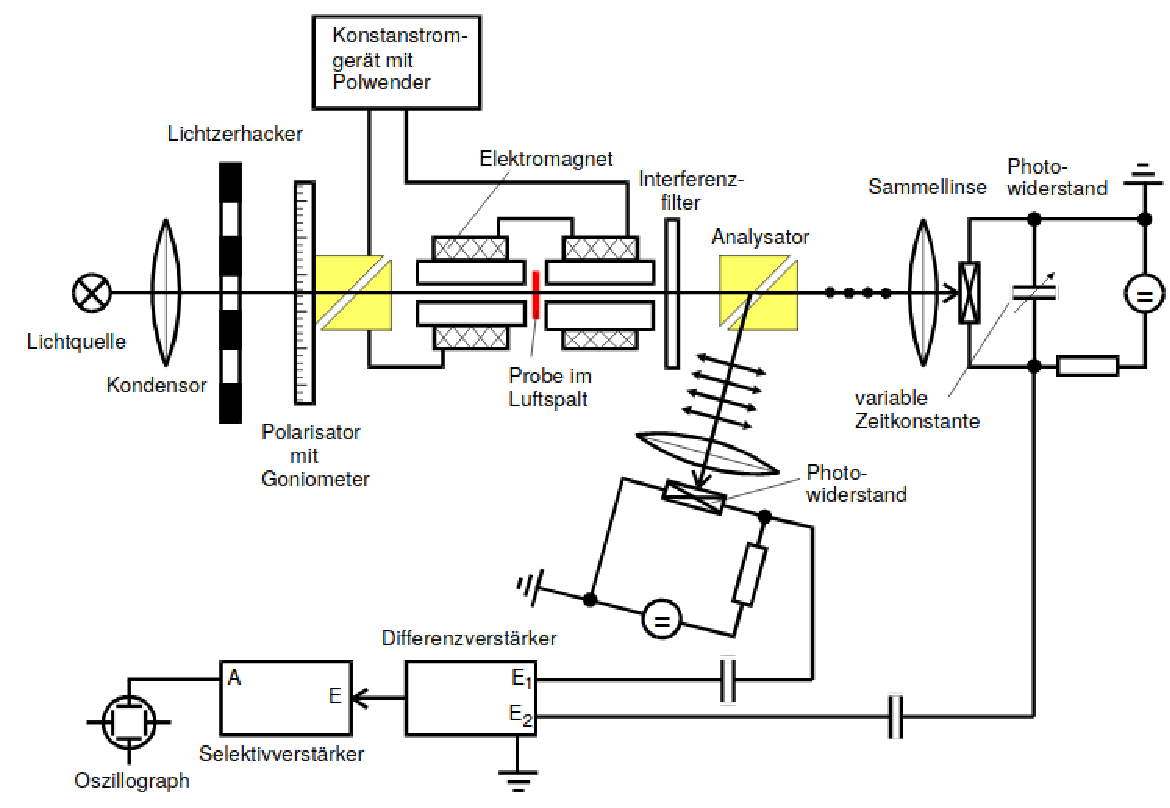
\includegraphics[width=0.9\textwidth]{figure/Aufbau.pdf}
    \caption{schematische Abbildung des Versuchsaufbaus \cite{sample}}
    \label{abb2}
\end{figure}

\section{Versuchsdurchführung}
\label{sec:Versuchsdurchführung}

Das Messprogramm ist in drei Schritte unterteilt.
Zunächst wird die Kraftflussdichte $B(z)$ in Strahlrichtung in der Nähe des 
Luftspaltes gemessen. Dafür wid die Kraftflussdichte für den Abstand $\SI{125}{\milli\meter}$
aufgenommen. Dann wird sich dem Luftspalt in $\SI{2}[\milli\meter}$ Schritten 
angenähert, bis der Abstand $\SI{107}{\milli\meter}$ erreicht ist. 
Zusätzlich wurden die Kraftflussdichten für die Abstände $\SI{114}{\milli\meter}$
und $\SI{116}{\milli\meter}$ aufgenommen, da bei zunächst bei $\SI{15}{\milli\meter}$
die maximale kraftflussdichte gemessen wurde.
Beim zweiten Messdurchlauf wird die Faraday-Rotaion für zwei unterschiedlich dicke 
n-dotierte GaAs-Proben gemessen. 
Die erste Probe hat eine Teilchendichte von $N = 1,2 \times \SI{10^{18}}{\centi\meter^{-3}}$ 
und eine Dicke von $L = \SI{1,36}{\milli\meter}$, während die zweite eine 
Teilchendichte von $N = 2,8 \times \SI{10^{18}}{\centi\meter^{-3}}$ 
und eine Dicke von $L = \SI{1,296}{\milli\meter}$ aufweist.
Das heißt, die Drehwinkel werden einmal für ein 
Magnetfeld in Strahlrichtung und ein Magnetfeld gegen Strahlrichtung bzgl. neun 
verschiedenen Wellenlängen im Bereich zwischen $\SI{1,06}{\micro\meter}$ 
und $\SI{2,65}{\micro\meter}$ gemessen.
Das letzte Messprogramm stellt eine Wiederholung des Zweiten für eine hochreine 
GaAs-Probe der Dicke $L = \SI{5,11}{\milli\meter}$ dar \cite{sample}.